\documentclass{article}
\usepackage{float}
\usepackage[polish]{babel}
\usepackage[utf8]{inputenc}
\usepackage{polski}
\usepackage{listings} %code environment
\frenchspacing
\setcounter{tocdepth}{2}
\usepackage{graphicx}
\graphicspath{ {images/} }

\lstdefinestyle{main}{
	keywords={
		after, always, causes, if, impossible, initially, observable, 
		partakes, releases, typically
    },
    keywordstyle={\bfseries},
    keywordstyle=[2]\textsc,
    frame=single,
}

\begin{document}
	
\begin{titlepage}

\newcommand{\HRule}{\rule{\linewidth}{0.5mm}}
\newcommand{\Action}[1]{\textsc{#1}}

\center

%----------------------------------------------------------------------------------------

\textsc{\LARGE Politechnika Warszawska}\\[5mm]
\textsc{\LARGE Wydział Matematyki i Nauk Informacyjnych}\\[3.5cm]
 
%----------------------------------------------------------------------------------------

\textsc{\Huge Reprezentacja wiedzy}\\[0.5cm]

%----------------------------------------------------------------------------------------

\HRule \\[0.4cm]
{ \LARGE \bfseries Programy działań z efektami domyślnymi}\\[2.5cm]
 
%----------------------------------------------------------------------------------------

\begin{flushright}
\Large \emph{Autorzy:}\\[0.5cm]
Dragan Łukasz\\
Flis Mateusz\\
Fusiara Marcin\\
Izert Piotr\\
Pielat Mateusz\\
Rząd Przemysław\\
Siry Roman\\
Waszkiewicz Piotr\\
Zawadzka Anna\\

\end{flushright}
%----------------------------------------------------------------------------------------

\vfill
{\large \today}\\[3cm]

\end{titlepage}
	
\newpage

\section{Opis zadania}

Zadaniem projektu jest opracowanie i zaimplementowanie języka akcji dla specyfikacji podanej klasy systemów dynamicznych oraz odpowiadający mu język kwerend.\\

System dynamiczny spełnia podane założenia:
\begin{enumerate}
\item Prawo inercji
\item Niedeterminizm i sekwencyjność działań
\item Pełna informacja o wszystkich akcjach i wszystkich ich skutkach bezpośrednich
\item Z każdą akcją związany jest:
\begin{enumerate}
\item Warunek początkowy (ew. true)
\item Efekt akcji
\item Jej wykonawca
\end{enumerate}
\item Skutki akcji:
\begin{enumerate}
\item Pewne (zawsze występują po zakończeniu akcji)
\item Domyślne (preferowane. Zachodzą po zakończeniu akcji, o ile nie jest wiadomym, że nie występują)
\end{enumerate}
\item Efekty akcji zależą od jej stanu, w którym akcja się zaczyna i wykonawcy tej akcji
\item W pewnych stanach akcje mogą być niewykonalne przez pewnych (wszystkich) wykonawców
\end{enumerate}

Programem działań nazywać będziemy ciąg $((A_{1},W_{1}), (A_{2},W_{2}), …, (A_{n},W_{n}))$, 
gdzie $A_{i}$ jest akcją, zaś $W_{i}$ jej wykonawcą lub $\epsilon$ (ktokolwiek).\\


Język kwerend zapewnia uzyskanie odpowiedzi na następujące pytania:
\begin{enumerate}
\item Czy podany program działań jest wykonywalny zawsze/kiedykolwiek?
\item Czy wykonanie podanego programu działań z dowolnego stanu spełniającego warunek $\pi$ prowadzi zawsze/kiedykolwiek/na ogół do stanu spełniającego warunek celu $\gamma$ ?
\item Czy z dowolnego stanu spełniającego warunek $\pi$ cel $\gamma$ jest osiągalny zawsze/kiedykolwiek/na ogół?
\item Czy wskazany wykonawca jest zaangażowany w realizację programu zawsze/kiedykolwiek?
\end{enumerate}


\section{Język akcji $\Omega$}

\subsection{Definicja języka}
$\Omega$ jest rodziną języków, w której każdy język $\mathcal{L}$ określony jest nad sygnaturą 
\begin{center}
$\Upsilon=(F,A,V)$
\end{center}
gdzie: 
\begin{itemize}
\item $F$ - niepusty zbiór zmiennych (fluenty)
\item $A$ - niepusty zbiór akcji
\item $V$ - niepusty zbiór wykonawców (aktorów), przy czym $\epsilon\in V$, gdzie $\epsilon$ oznacza kogokolwiek
\end{itemize}

\subsection{Syntaktyka języka}
Przed przystąpieniem do opisu typów zdań wprowadzone zostanie oznaczenie listy wykonawców $W \in V; W=(w_{1}, w_{2}, \dots, w_{n})$ które reprezentuje listę dopuszczalnych wykonawców danej akcji. Dodatkowo możliwy jest zapis \textit{negatywny} w postaci $W=(\neg w_{1}, \neg w_{2}, \dots, \neg w_{n})$ oznaczający wyłączenie wymienionych wykonawców z możliwości wykonywania danej akcji.
W języku  $\Omega$ występują następujące typy zdań:
\begin{itemize}
\item {\large\texttt{initially $\alpha$}}\\
formuła $\alpha$ zachodzi w stanie początkowym
\item {\large\texttt{$\alpha$ after $(A_{1},W_{1}), ..., (A_{n},W_{n})$}}\\
formuła $\alpha$ zachodzi po wykonaniu sekwencji $(A_{1},W_{1}), ..., (A_{n},W_{n})$, gdzie $A_{i}$ jest akcją, zaś $W_{i}$ jej niepustą listą wykonawców
\item {\large\texttt{$(A,W)$ causes $\alpha$ if $\pi$}}\\
skutkiem wykonania akcji $A$ przez któregokolwiek z wykonawców $W$ w stanie spełniającym warunek $\pi$ jest stan, w którym spełniona jest formuła $\alpha$. Przy czym:
\begin{itemize}
    \item Jeśli $\pi \Leftrightarrow \top$, to powyższe zdanie zapisujemy:\\
    {\large\texttt{$(A,W)$ causes $\alpha$ }}\\
    oznacza to, że skutkiem wykonania akcji $A$ przez któregokolwiek z wykonawców $W$ jest stan, w którym spełniona jest formuła $\alpha$
    \item Jeśli $\alpha \Leftrightarrow \perp$, to powyższe zdanie zapisujemy:\\
    {\large\texttt{impossible $(A,W)$ if $\pi$}}\\
    co oznacza, że niemożliwe jest wykonanie akcji $A$ przez któregokolwiek z wykonawców $W$ w stanie spełniającym warunek $\pi$
\end{itemize}
\item {\large\texttt{observable $\alpha$ after $(A_{1},W_{1}), ..., (A_{n},W_{n})$}}\\
po wykonaniu sekwencji $(A_{1},W_{1}), ..., (A_{n},W_{n})$, gdzie $A_{i}$ jest akcją, zaś $W_{i}$ jej potencjalnymi wykonawcami, w stanie początkowym może (ale nie musi) zachodzić formuła $\alpha$
\item {\large\texttt{$(A,W)$ releases $f$ if $\pi$}}\\
wykonanie akcji $A$ przez któregokolwiek z wykonawców $W$ w stanie spełniającym warunek $\pi$ może (ale nie musi) zmienić wartość zmiennej $f$
\item {\large\texttt{$(A,W)$ typically causes $\alpha$ if $\pi$}}\\
skutkiem wykonania akcji $A$ przez któregokolwiek z wykonawców $w$ w stanie spełniającym warunek $\pi$ na ogół jest stan, w którym spełniona jest formuła $\alpha$
\item {\large\texttt{typically $\alpha$ after $(A_{1},W_{1}), ..., (A_{n},W_{n})$}}\\
formuła $\alpha$ na ogół zachodzi po wykonaniu sekwencji $(A_{1},W_{1}), ..., (A_{n},W_{n})$, gdzie $A_{i}$ jest akcją, zaś $W_{i}$ listą jej potencjalnych wykonawców
\item {\large\texttt{always $\alpha$}}\\
formuła $\alpha$ jest spełniona w każdym stanie
\end{itemize}
gdzie $\alpha$ jest dowolną kombinacją zmiennych (fluentów): 
\begin{center}
$\alpha= f | \alpha | \neg\alpha | \alpha_{1} \land \alpha_{2} | \alpha_{1} \lor \alpha_{2} | \alpha_{1} \to \alpha_{2} | \alpha_{1} \leftrightarrow \alpha_{2} $
\end{center}

\subsection{Przykłady} 
\subsubsection{Gotujący John}


\textit{John jest entuzjastą gotowania i bardzo lubi jeść. Zakładamy, że początkowo jest głodny, jego lodówka jest pusta, nie ma on żadnego gotowego posiłku i w jego kuchni panuje porządek. Jeśli John jest głodny, to jest też zły. Nie może jednak nic zjeść, jeśli nie ma co. Niemożliwym jest także ugotowanie posiłku, jeśli lodówka Johna jest pusta. Aby ją uzupełnić John idzie na zakupy. Zakupy również często powodują, że John ma lepszy humor. John może teraz coś ugotować, lecz jeśli jest zły to na ogół powoduje to ogromy chaos w kuchni. Zdolności kulinarne Johna są na tyle duże, że zawsze wyjdzie mu posiłek, który jest zdatny do jedzenia. John lubi duże porcje, więc możliwe, że po ugotowaniu posiłku znowu ma pustą lodówkę. Jest też takim łakomczuchem, że nie zostawia sobie nic na później i zjada cały posiłek. Po zjedzeniu głód mija, a humor Johna się poprawia.}

\bigskip
\lstset{
	style=main,
	keywords=[2]{Eat, Shop, Cook},
}
\begin{lstlisting}[mathescape=true]
initially hungry $\wedge$ angry
initially emptyFridge $\wedge$ $\neg$hasMeal $\wedge$ $\neg$chaos 
impossible (Eat,John) if $\neg$hasMeal 
impossible (Cook,John) if emptyFridge
(Shop,John) causes $\neg$emptyFridge
(Shop,John) releases angry if angry
(Cook,John) typically causes chaos if angry
(Cook,John) causes hasMeal 
(Cook,John) releases emptyFridge 
(Eat,John) causes $\neg$hasMeal $\wedge$ $\neg$hungry $\wedge$ $\neg$angry
\end{lstlisting}

\subsubsection{Programiści Fred i Bill}


\textit{Farmer Bill i indyk Fred pracują razem nad pewnym projektem programistycznym. Zakładamy, że początkowo kod jest czytelny i kompilowalny. Bill to niedoświadczony programista, więc gdy dopisze on jakiś fragment cały kod przestaje być czytelny, a nierzadko przestaje się też kompilować. Indyk Fred jest z kolei weteranem branży IT, więc jego kod kompiluje się zawsze (gdy pracuje on z czytelnym kodem) lub prawie zawsze (gdy kod jest nieczytelny). W razie potrzeby Fred refaktoryzuje cały kod, dzięki czemu poprawia się jego czytelność. Bill i Fred zgodnie ustalili, że nie będą dopisywać nowych fragmentów kodu jeżeli dotychczasowy się nie kompiluje. W takim wypadku któryś z nich musi go najpierw zdebugować (co potrafi każdy programista mając odpowiednio dużo czasu).}

\bigskip
\lstset{
	style=main,
	keywords=[2]{Code, Debug, Refactor},
}
\begin{lstlisting}[mathescape=true]
initially compiles $\wedge$ cleanCode
(Code,Bill) causes $\neg$cleanCode
(Code,Bill) releases compiles if compiles
(Code,Fred) causes compiles if cleanCode
(Code,Fred) typically causes compiles if $\neg$cleanCode
(Refactor,Fred) causes cleanCode
(Debug,$\epsilon$) causes compiles
impossible (Code,$\epsilon$) if $\neg$compiles
\end{lstlisting}

\subsubsection{Alicja w krainie czarów}


\textit{Alicja może być pomniejszona, lub być swojego normalnego, wysokiego wzrostu. Początkowo Alicja jest wysoka. Wypicie Eliksiru pomnniejsza Alicję, natomiast zjedzenie Ciastka ją powiększa.
\\
Kot z Cheshire nigdy nie zje Ciastka, a wypicie przez niego Eliksiru zwykle go ujawnia, jeśli jest niewidzialny. Kot początkowo jest niewidzialny.
\\
Kapelusznik początkowo nie jest szalony. Wypicie Eliksiru może doprowadzić go do szaleństwa, a zjedzenie Ciastka zwykle powoduje powrót do zdrowych zmysłów.
\\
Ciastko jest tylko jedno więc znika po jego zjedzeniu i nie można próbować go zjeść, natomiast duża, nieprzeźroczysta butelka Eliksiru nie musi być pusta po napiciu się z niej.
\\
Biały Królik nigdy nie zje ciastka, a wypicie przez niego Eliksiru powoduje magiczne pojawienie się Ciastka z powrotem.
\\
Początkowo Ciastko jest dostępne, a butelka pełna Eliksiru.}

\bigskip
\lstset{
	style=main,
	keywords=[2]{Drink, Eat},
}
\begin{lstlisting}[mathescape=true, breaklines=true]
initially $\neg$aliceSmall  $\wedge$ $\neg$hatterMad $\wedge$ $\neg$catVisible
initially cakeExists $\wedge$ elixirExists
(Drink,Alice) causes aliceSmall if elixirExists
(Eat,Alice) causes $\neg$aliceSmall
impossible (Eat,Cat)
(Drink,Cat) typically causes catVisible if elixirExists
(Drink,Hatter) releases hatterMad if $\neg$hatterMad $\wedge$ elixirExists
(Eat,Hatter) typically causes $\neg$hatterMad if hatterMad
(Eat,$\epsilon$) causes $\neg$cakeExists
impossible (Eat,$\epsilon$) if $\neg$cakeExists
(Drink,$\epsilon$) releases elixirExists if elixirExists
impossible (Eat,Rabbit)
(Drink,Rabbit) causes cakeExists if elixirExists
\end{lstlisting}

\subsection{Semantyka języka} 

\subsubsection{Stan}
Stanem będziemy nazywać dowolną funkcję $\sigma:F\to \{1,0\}$, która przypisuje zmiennym wartości logiczne. Jeśli $\sigma(f)=1$, to znaczy, że zmienna $f$ zachodzi w stanie $\sigma$. Funkcję tę można rozszerzyć na zbiór wszystkich formuł nad zbiorem zmiennych $F$ według zasad obowiązujących w klasycznej logice zdań.

\subsubsection{Struktura}
Strukturą nazywamy układ $S=(\Sigma, \sigma_{0}, ResAb, ResN)$, gdzie:
\begin{itemize}
\item $\Sigma$ - zbiór stanów
\item $\sigma_{0} \in \Sigma$ - stan początkowy
\item $ResAb, ResN$ : $A\times W \times \Sigma \to 2^{\Sigma}$ są funkcjami przejść. $ResAb$ jest funkcją przejść nietypowych, $ResN$ jest funkcją przejść typowych oraz $ResAb \cap ResN= \emptyset$ 
\end{itemize}

\subsubsection{Dziedzina}
Niech $\mathcal{L}$ będzie językiem z rodziny $\Omega$. Dziedziną akcji nazywamy niepusty zbiór $D$ zdań języka $\mathcal{L}$.

\subsubsection{Model dziedziny}
W celu zdefiniowania pojęcia modelu dziedziny wprowadzone zostaną następujące funkcje pomocnicze:
\begin{enumerate}
	\item $Res_{0}$ : $A \times W \times \Sigma \to 2^{\Sigma}$ konstruowane na podstawie zdań efektów akcji.
	\[ \forall_{a \in A, w \in W, \sigma \in \Sigma} Res_{0}(a,w,\sigma) = \{\sigma' \in \Sigma: ((a, w) \textbf{ causes } \alpha \textbf{ if } \pi) \in D \land (\sigma \models \pi) \Rightarrow (\sigma' \models \alpha) \}  \]
	Oznacza to, że $Res_{0}$ konstruuje się bez minimalizacji zmian.
	\item Funkcję $Res^{-}$ wyznacza się stosując minimalizację zmian.
	\item Funkcję $Res_{0}^{+} : A \times W \times \Sigma \to 2^{\Sigma}$ spełniającą warunek $\forall_{a \in A, w \in W, \sigma \in \Sigma}$:
	\[ Res_{0}^{+}(a, w,\sigma) = \]
	\[ \{\sigma' \in Res_{0}(a, w,\sigma) : ((a, w) \textbf{ typically causes } \beta \textbf{ if } \pi) \in D \land (\sigma \models \varphi) \Rightarrow (\sigma' \models \beta) \}  \]
\end{enumerate}

Niech D będzie dziedziną akcji języka $\Omega$ i niech $S=(\Sigma, \sigma_{0}, ResAb, ResN)$ będzie strukturą dla $\Omega$. Mówimy, że S jest modelem D $\leftrightarrow$ spełnione są warunki:
\begin{itemize}
	\item $\Sigma$ jest zbiorem stanów z dziedziny D
	\item każde zdanie obserwacji i każde zdanie wartości z dziedziny D jest prawdziwe w S
	\item $\forall_{ a \in A, w \in W, \sigma \in \Sigma } ResN(a, w, \sigma)$ jest zbiorem tych wszystkich stanów $\sigma' \in Res_{0}^{+}(a, w, \sigma)$, dla których zbiory $New(a, w, \sigma, \sigma')$ są minimalne
	\item $\forall_{a \in A, w \in W, \sigma \in \Sigma} ResAb(a, w, \sigma) = Res^{-}(a, w, \sigma) | ResN(a, w, \sigma)$
\end{itemize}
Warto zwrócić uwagę na to, że skutki \textit{pewne} dla akcji traktowane są jak \textit{typowe}.

\subsubsection{Funkcja przejścia}
Niech $S=(\Sigma,\sigma_{0},ResAb,ResN)$ będzie strukturą dla języka. Konstrukcja funkcji $\Psi_{S} : (A \times W)^{*} \times \Sigma \to \Sigma$ wygląda następująco:
\begin{itemize}
	\item $\Phi_{S}(a,\epsilon,\sigma)=\sigma$ gdzie $\epsilon$ oznacza ciąg pusty
	\item jeśli $\Phi_{S}(((a_{1}, W_{1}), \dots, (a_{n}, W_{n})),\sigma)$ jest określona to
	\[\Phi_{S}(((a_{1}, W_{1}), \dots, (a_{n}, W_{n})),\sigma) \in ResAb((a_{n}, W_{n}), \Phi_{S}((a_{1}, W_{1}),\dots,(a_{n-1}, W_{n-1}))) \]
	\[ \cup ResN((a_{n}, W_{n}), \Phi_{S}((a_{1}, W_{1}),\dots,(a_{n-1}, W_{n-1})))\]
\end{itemize}
\subsection{Konstrukcja modeli}\mbox{}\\
Przy wyznaczaniu funkcji przejścia $ResN$ i $ResAb$ stosujemy zasadę zaczerpniętą z języka $AR$, tj. stany niedopuszczalne są eliminowane przed minimalizacją zmian.
\subsection{Scenariusz}
Scenariuszem nazywamy skończony ciąg par akcja-wykonawca:
\begin{center}
$SC=((A_1,W_1),(A_2,W_2),...,(A_n,W_n))$
\end{center}
\textbf{Przykład:}
\lstset{
	style=main,
	keywords=[2]{Eat, Shop, Cook},
}
\begin{lstlisting}[mathescape=true]
(Shop,John), (Cook,John), (Eat,John)
\end{lstlisting}
Powyższy scenariusz mówi, iż John wykonał kolejno akcje: \texttt{SHOP, COOK, EAT}.

\newpage
\subsection{Przykłady}
\subsubsection{Gotujący John}

Rozważmy następującą dziedzinę:
\bigskip
\lstset{
	style=main,
	keywords=[2]{Eat, Shop, Cook},
}
\begin{lstlisting}[mathescape=true]
initially hungry $\wedge$ $\neg$hasMeal 
impossible (Eat,John) if $\neg$hasMeal 
(Cook,John) typically causes hasMeal
(Eat,John) causes $\neg$hasMeal 
(Eat,John) releases hungry if hungry
\end{lstlisting}
Zbiór stanów dopuszczalnych to $\Sigma=\{\sigma_{0},\sigma_{1},\sigma_{2},\sigma_{3}\}$, gdzie:\\
$\sigma_{0}=\{h,\neg m\}$, $\sigma_{1}=\{h, m\}$, $\sigma_{2}=\{\neg h, m\}$, $\sigma_{3}=\{\neg h,\neg m\}$, zaś $h$ i $m$ oznaczają odpowiednio $hungry$ i $hasMeal$.\\

\begin{minipage}[t]{0.5\textwidth}
$Res_{0}(\textsc{Cook},John,\sigma_{0})=\Sigma$\\
$New(\textsc{Cook},John,\sigma_{0},\sigma_{0})=\emptyset$\\
$New(\textsc{Cook},John,\sigma_{0},\sigma_{1})=\{m\}$\\
$New(\textsc{Cook},John,\sigma_{0},\sigma_{2})=\{\neg h,m\}$\\
$New(\textsc{Cook},John,\sigma_{0},\sigma_{3})=\{\neg h\}$\\
$Res^{-}(\textsc{Cook},John,\sigma_{0})=\{\sigma_{0}\}$\\
$Res_{0}^{+}(\textsc{Cook},John,\sigma_{0})=\{\sigma_{1},\sigma_{2}\}$\\\\
$ResN(\textsc{Cook},John,\sigma_{0})=\{\sigma_{1}\}$\\
$ResAb(\textsc{Cook},John,\sigma_{0})=\{\sigma_{0}\}$\\\\
$Res_{0}(\textsc{Eat},John,\sigma_{0})=\emptyset$,\\ 
ponieważ: \\impossible $(\textsc{Eat},John)$ if $\neg$hasMeal\\\\
$ResN(\textsc{Eat},John,\sigma_{0})=\emptyset$,\\ 
$ResAb(\textsc{Eat},John,\sigma_{0})=\emptyset$,\\ 

\end{minipage}
\begin{minipage}[t]{0.5\textwidth}
$ResN(\textsc{Cook},John,\sigma_{1})=\{\sigma_{1}\}$\\
$ResAb(\textsc{Cook},John,\sigma_{1})=\emptyset$\\\\
$ResN(\textsc{Eat},John,\sigma_{1})=\{\sigma_{0},\sigma_{3}\}$\\ 
$ResAb(\textsc{Eat},John,\sigma_{1})=\emptyset$\\\\
$ResN(\textsc{Cook},John,\sigma_{2})=\{\sigma_{2}\}$\\
$ResAb(\textsc{Cook},John,\sigma_{2})=\emptyset$\\\\
$ResN(\textsc{Eat},John,\sigma_{2})=\{\sigma_{3}\}$\\ 
$ResAb(\textsc{Eat},John,\sigma_{2})=\emptyset$\\\\
$ResN(\textsc{Cook},John,\sigma_{3})=\{\sigma_{2}\}$\\
$ResAb(\textsc{Cook},John,\sigma_{3})=\{\sigma_{3}\}$\\\\
$ResN(\textsc{Eat},John,\sigma_{3})=\emptyset$\\ 
$ResAb(\textsc{Eat},John,\sigma_{3})=\emptyset$\\\\
\end{minipage}
\begin{figure}[H]
\centering
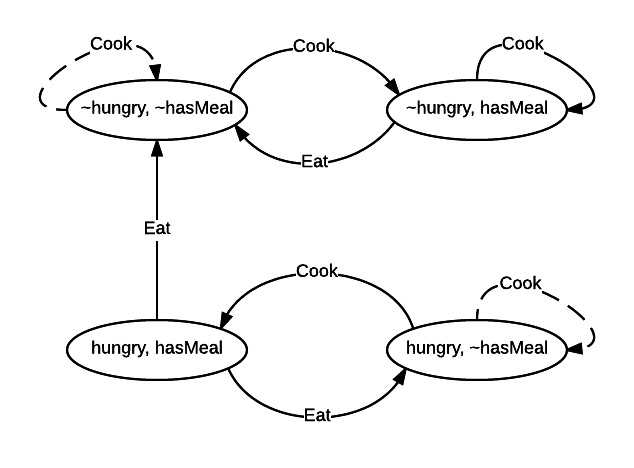
\includegraphics[scale=1]{John}
\caption{Graf zależności - gotujący John}
\end{figure}


\subsubsection{Programista Fred}

Rozważmy następującą dziedzinę:
\bigskip
\lstset{
	style=main,
	keywords=[2]{Code, Debug, Refactor},
}
\begin{lstlisting}[mathescape=true]
initially compiles $\wedge$ cleanCode
(Code,Fred) causes $\neg$cleanCode
(Code,Fred) causes compiles if cleanCode
(Code,Fred) typically causes compiles if $\neg$cleanCode
(Refactor,Fred) causes cleanCode
(Debug,Fred) causes compiles
impossible (Code,Fred) if $\neg$compiles
\end{lstlisting}
Zbiór stanów dopuszczalnych to $\Sigma=\{\sigma_{0},\sigma_{1},\sigma_{2},\sigma_{3}\}$, gdzie:\\
$\sigma_{0}=\{cm,cc\}$, $\sigma_{1}=\{cm,\neg cc\}$, $\sigma_{2}=\{\neg cm,cc\}$, $\sigma_{3}=\{\neg cm,\neg cc\}$, zaś $cm$ i $cc$ oznaczają odpowiednio $compiles$ i $cleanCode$.\\

\begin{minipage}[t]{0.5\textwidth}
$Res_{0}(\textsc{Code},Fred,\sigma_{0}) = \{\sigma_{1}\}$\\
$New(\textsc{Code},Fred,\sigma_{0},\sigma_{1}) = \{cc\}$\\
$Res^{-}(\textsc{Code},Fred,\sigma_{0}) = \{\sigma_{1}\}$\\
$Res_{0}^{+}(\textsc{Code},Fred,\sigma_{0}) = \{\sigma_{1}\}$\\\

$ResN(\textsc{Code},Fred,\sigma_{0}) = \{\sigma_{1}\}$\\
$ResAb(\textsc{Code},Fred,\sigma_{0}) = \emptyset$\\

$Res_{0}(\textsc{Code},Fred,\sigma_{1}) = \{\sigma_{1},\sigma_{3}\}$\\
$New(\textsc{Code},Fred,\sigma_{1},\sigma_{1}) = \emptyset$\\
$New(\textsc{Code},Fred,\sigma_{1},\sigma_{3}) = \{cm\}$\\
$Res^{-}(\textsc{Code},Fred,\sigma_{1}) = \{\sigma_{1}\}$\\
$Res_{0}^{+}(\textsc{Code},Fred,\sigma_{1}) = \{\sigma_{1}\}$\\\

$ResN(\textsc{Code},Fred,\sigma_{1}) = \{\sigma_{1}\}$\\
$ResAb(\textsc{Code},Fred,\sigma_{1}) = \emptyset$\\\

$ResN(\textsc{Debug},Fred,\sigma_{0}) = \{\sigma_{0}\}$\\
$ResAb(\textsc{Debug},Fred,\sigma_{0}) = \emptyset$\\\
\end{minipage}
\begin{minipage}[t]{0.5\textwidth}
$ResN(\textsc{Debug},Fred,\sigma_{1}) = \{\sigma_{1}\}$\\
$ResAb(\textsc{Debug},Fred,\sigma_{1}) = \emptyset$\\\

$ResN(\textsc{Debug},Fred,\sigma_{2}) = \{\sigma_{0}\}$\\
$ResAb(\textsc{Debug},Fred,\sigma_{2}) = \emptyset$\\\

$ResN(\textsc{Debug},Fred,\sigma_{3}) = \{\sigma_{1}\}$\\
$ResAb(\textsc{Debug},Fred,\sigma_{3}) = \emptyset$\\\

$ResN(\textsc{Refactor},Fred,\sigma_{0}) = \{\sigma_{0}\}$\\
$ResAb(\textsc{Refactor},Fred,\sigma_{0}) = \emptyset$\\\

$ResN(\textsc{Refactor},Fred,\sigma_{1}) = \{\sigma_{0}\}$\\
$ResAb(\textsc{Refactor},Fred,\sigma_{1}) = \emptyset$\\\

$ResN(\textsc{Refactor},Fred,\sigma_{2}) = \{\sigma_{2}\}$\\
$ResAb(\textsc{Refactor},Fred,\sigma_{2}) = \emptyset$\\\

$ResN(\textsc{Refactor},Fred,\sigma_{3}) = \{\sigma_{2}\}$\\
$ResAb(\textsc{Refactor},Fred,\sigma_{3}) = \emptyset$\\\\
\end{minipage}
\begin{figure}[H]
\centering
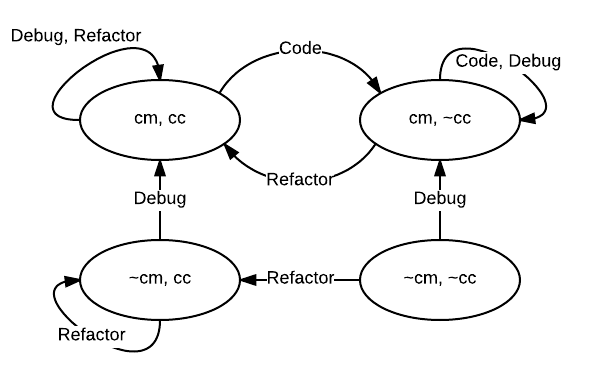
\includegraphics[scale=1]{Programmers}
\caption{Graf zależności - Programista Fred}
\end{figure}
\newpage
\subsubsection{Kapelusznik w krainie czarów}

Rozważmy następującą dziedzinę:
\bigskip
\lstset{
	style=main,
	keywords=[2]{Eat, Drink},
}
\begin{lstlisting}[mathescape=true]
initially $\neg$hatterMad $\wedge$ cakeExists $\wedge$ elixirExists
(Drink,Hatter) causes hatterMad if elixirExists
(Eat,Hatter) typically causes $\neg$hatterMad if hatterMad
impossible (Eat,Hatter) if $\neg$cakeExists
(Drink,Hatter) releases elixirExists if elixirExists
(Eat,Hatter) causes $\neg$cakeExists
\end{lstlisting}
Zbiór stanów dopuszczalnych to $\Sigma=\{\sigma_{0},\sigma_{1},\sigma_{2},\sigma_{3},\sigma_{4},\sigma_{5},\sigma_{6},\sigma_{7}\}$, gdzie:\\
$\sigma_{0}=\{\neg h,c, e\}$, $\sigma_{1}=\{h, c, e\}$, $\sigma_{2}=\{h, \neg c, e\}$, $\sigma_{3}=\{\neg h,\neg c, e\}, \sigma_{4}=\{h,\neg c, \neg e\}$, $\sigma_{5}=\{h, c, \neg e\}$, $\sigma_{6}=\{\neg h, c, \neg e\}$, $\sigma_{7}=\{\neg h,\neg c, \neg e\}$, zaś $h$, $c$, $e$ oznaczają odpowiednio $hatterMad$, $cakeExists$, $elixirExists$.\\\\
$Res_{0}(\textsc{Drink},Hatter,\sigma_{0})=\{\sigma_{1}, \sigma_{2}, \sigma_{4}, \sigma_{5}\}$\\
$New(\textsc{Drink},Hatter,\sigma_{0},\sigma_{1})=\{h, e\}$\\
$New(\textsc{Drink},Hatter,\sigma_{0},\sigma_{2})=\{h, c, e\}$\\
$New(\textsc{Drink},Hatter,\sigma_{0},\sigma_{4})=\{h, c, e\}$\\
$New(\textsc{Drink},Hatter,\sigma_{0},\sigma_{5})=\{h, e\}$\\
$Res^{-}(\textsc{Drink},Hatter,\sigma_{0})=\{\sigma_{1}, \sigma_{5}\}$\\
$Res_{0}^{+}(\textsc{Drink},Hatter,\sigma_{0})=\{\sigma_{1}, \sigma_{2}, \sigma_{4}, \sigma_{5}\}$\\\\
$ResN(\textsc{Drink},Hatter,\sigma_{0})=\{\sigma_{1}, \sigma_{5}\}$\\
$ResAb(\textsc{Drink},Hatter,\sigma_{0})=\emptyset$\\\\
$Res_{0}(\textsc{Eat},Hatter,\sigma_{0})=\{\sigma_{1}, \sigma_{2}, \sigma_{4}, \sigma_{5}\}$\\
$New(\textsc{Eat},Hatter,\sigma_{0},\sigma_{2})=\{h, c\}$\\
$New(\textsc{Eat},Hatter,\sigma_{0},\sigma_{3})=\{c\}$\\
$New(\textsc{Eat},Hatter,\sigma_{0},\sigma_{4})=\{h, c, e\}$\\
$New(\textsc{Eat},Hatter,\sigma_{0},\sigma_{7})=\{c, e\}$\\
$Res^{-}(\textsc{Eat},Hatter,\sigma_{0})=\{\sigma_{3}\}$\\
$Res_{0}^{+}(\textsc{Eat},Hatter,\sigma_{0})=\{\sigma_{1}, \sigma_{2}, \sigma_{4}, \sigma_{5}\}$\\\\
$ResN(\textsc{Eat},Hatter,\sigma_{0})=\{\sigma_{3}\}$\\
$ResAb(\textsc{Eat},Hatter,\sigma_{0})=\emptyset$\\\\
$ResN(\textsc{Drink},Hatter,\sigma_{1})=\{\sigma_{1}, \sigma_{5}\}$\\
$ResAb(\textsc{Drink},Hatter,\sigma_{1})=\emptyset$\\\\
$ResN(\textsc{Eat},Hatter,\sigma_{1})=\{\sigma_{3}\}$\\
$ResAb(\textsc{Eat},Hatter,\sigma_{1})=\{\sigma_{2}\}$\\\\
$ResN(\textsc{Drink},Hatter,\sigma_{2})=\{\sigma_{2}, \sigma_{4}\}$\\
$ResAb(\textsc{Drink},Hatter,\sigma_{2})=\emptyset$\\\\
$ResN(\textsc{Eat},Hatter,\sigma_{2})=\emptyset$\\
$ResAb(\textsc{Eat},Hatter,\sigma_{2})=\emptyset$\\\\
$ResN(\textsc{Drink},Hatter,\sigma_{3})=\{\sigma_{2}, \sigma_{7}\}$\\
$ResAb(\textsc{Drink},Hatter,\sigma_{3})=\emptyset$\\\\
$ResN(\textsc{Eat},Hatter,\sigma_{3})=\emptyset$\\
$ResAb(\textsc{Eat},Hatter,\sigma_{3})=\emptyset$\\\\
$ResN(\textsc{Drink},Hatter,\sigma_{4})=\{\sigma_{4}\}$\\
$ResAb(\textsc{Drink},Hatter,\sigma_{4})=\emptyset$\\\\
$ResN(\textsc{Eat},Hatter,\sigma_{4})=\emptyset$\\
$ResAb(\textsc{Eat},Hatter,\sigma_{4})=\emptyset$\\\\
$ResN(\textsc{Drink},Hatter,\sigma_{5})=\{\sigma_{5}\}$\\
$ResAb(\textsc{Drink},Hatter,\sigma_{5})=\emptyset$\\\\
$ResN(\textsc{Eat},Hatter,\sigma_{5})=\{\sigma_{7}\}$\\
$ResAb(\textsc{Eat},Hatter,\sigma_{5})=\{\sigma_{4}\}$\\\\
$ResN(\textsc{Drink},Hatter,\sigma_{6})=\{\sigma_{6}\}$\\
$ResAb(\textsc{Drink},Hatter,\sigma_{6})=\emptyset$\\\\
$ResN(\textsc{Eat},Hatter,\sigma_{6})=\{\sigma_{7}\}$\\
$ResAb(\textsc{Eat},Hatter,\sigma_{6})=\emptyset$\\\\
$ResN(\textsc{Drink},Hatter,\sigma_{7})=\{\sigma_{7}\}$\\
$ResAb(\textsc{Drink},Hatter,\sigma_{7})=\emptyset$\\\\
$ResN(\textsc{Eat},Hatter,\sigma_{7})=\emptyset$\\
$ResAb(\textsc{Eat},Hatter,\sigma_{7})=\emptyset$\\

\begin{figure}[H]
\centering
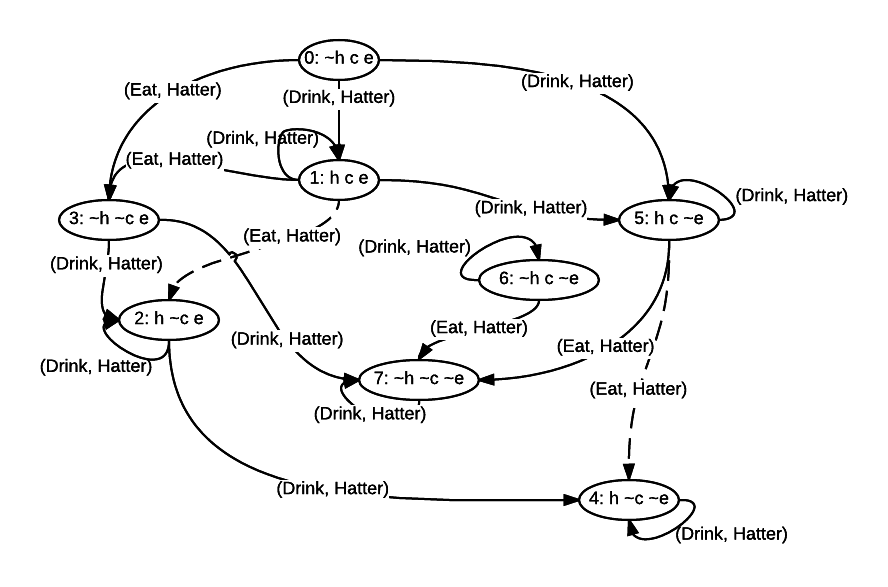
\includegraphics[scale=1]{Alice}
\caption{Graf zależności - Kapelusznik w krainie czarów}
\end{figure}


\newpage
\section{Język kwerend}
W celu zadawania pytań dotyczących świata opisanego powyższym językiem został stworzony język kwerend. Składa się on z następujących pytań (kwerend) pozwalających uzyskać odpowiedzi typu PRAWDA/FAŁSZ:

\subsection{Syntaktyka kwerend}
\begin{itemize}
\item Q1 - Czy podany program działań jest wykonywalny zawsze/kiedykolwiek?\\
% TODO: A może executable from ...?
{\large\texttt{always/ever executable $SC$}} \\
Zdanie to mówi, że wykonując podany ciąg akcji $SC$ z dowolnego, niesprzecznego stanu zawsze(\texttt{always}) osiągnięty zostanie niesprzeczny stan końcowy, lub istnieje przynajmniej jedna ścieżka z dowolnego z tych stanów do poprawnego stanu wynikowego(\texttt{ever}).


\item Q2 - Czy wykonanie podanego programu działań z dowolnego stanu spełniającego warunek $\pi$ prowadzi zawsze/kiedykolwiek/na ogół do stanu spełniającego warunek celu $\gamma$ ?\\
{\large\texttt{always/ever/typically accessible $\gamma$ if $\pi$ when $SC$}} \\
Podobnie jak Q1 zdanie to mówi, że osiągnięcie legalnego stanu końcowego spełniającego warunek $\gamma$, startując ze stanu spełniającego warunek $\pi$, nastąpi niezależnie od wybranego punktu początkowego(\texttt{always}), przynajmniej raz(\texttt{ever}), lub zawsze pod warunkiem wyboru zawsze ścieżki akcji domyślnej(\texttt{typically}).



\item Q3 - Czy z dowolnego stanu spełniającego warunek $\pi$ cel $\gamma$ jest osiągalny zawsze/kiedykolwiek/na ogół?\\
{\large\texttt{always/ever/typically accessible $\gamma$ if $\pi$}}


\item Q4 - Czy wskazany wykonawca jest zaangażowany w realizację programu zawsze/kiedykolwiek?\\
{\large\texttt{always/ever partakes $w$ when $SC$}} \\

\end{itemize}


\subsection{Semantyka kwerend}
Kwerenda Q jest prawdziwa względem dziedziny D wtedy i tylko wtedy gdy
\begin{enumerate}
	\item Jeśli Q jest zdaniem typu Q1:
	\begin{itemize}
		\item z warunkiem \texttt{always}: $\forall_{S=(\Sigma, \sigma_{0}, ResAb, ResN) \in D}\forall_{\Phi_{S}} \Phi_{S}(((A_{1}, W_{1}), \dots, (A_{n}, W_{n})), \sigma_{0})$ jest określona
		\item z warunkiem \texttt{ever}: 
		$\forall_{S=(\Sigma, \sigma_{0}, ResAb, ResN) \in D}\exists_{\Phi_{S}} \Phi_{S}(((A_{1}, W_{1}), \dots, (A_{n}, W_{n})), \sigma_{0})$ jest określona
	\end{itemize}
	\item Jeśli Q jest zdaniem typu Q2:
	\begin{itemize}
		\item z warunkiem \texttt{always}: 
		$\forall_{S=(\Sigma, \sigma_{0}, ResAb, ResN) \in D, \sigma_{0} \models \pi, SC=((A_{1}, W_{1}), \dots, (A_{n}, W_{n}))} \Phi_{S}(SC, \sigma_{0})$ jest określona dla każdej funkcji $\Phi_{S}$ oraz $\Phi_{S}(SC, \sigma_{0}) \models \gamma$
		\item z warunkiem \texttt{ever}:
		$\exists_{S=(\Sigma, \sigma_{0}, ResAb, ResN) \in D, \sigma_{0} \models \pi, SC=((A_{1}, W_{1}), \dots, (A_{n}, W_{n}))} \Phi_{S}$ oraz $\Phi_{S}(SC, \sigma_{0}) \models \gamma$
		\item z warunkiem \texttt{typically}:
		% TODO: Nie jestem pewien tego Res0+
		$\forall_{S=(\Sigma, \sigma_{0}, Res_{0}^{+}) \in D, \sigma_{0} \models \pi, SC=((A_{1}, W_{1}), \dots, (A_{n}, W_{n}))} \Phi_{S}(SC, \sigma_{0})$ jest określona dla funkcji $\Phi_{S}$ oraz $\Phi_{S}(SC, \sigma_{0}) \models \gamma$
	\end{itemize}
	
	\item Jeśli Q jest zdaniem typu Q3:
	\begin{itemize}
		\item z warunkiem \texttt{always}: 
		$\forall_{S=(\Sigma, \sigma_{0}, ResAb, ResN) \in D, \sigma_{0} \models \pi} \forall_{SC=((A_{1}, W_{1}), \dots, (A_{n}, W_{n}))}$ taki, że $\Phi_{S}(SC, \sigma_{0})$ jest określona dla każdej funkcji $\Phi_{S}$ oraz $\Phi_{S}(SC, \sigma_{0}) \models \gamma$
		\item z warunkiem \texttt{ever}:
		$\forall_{S=(\Sigma, \sigma_{0}, ResAb, ResN) \in D, \sigma_{0} \models \pi} \exists_{SC=((A_{1}, W_{1}), \dots, (A_{n}, W_{n}))}$ taki, że $\Phi_{S}(SC, \sigma_{0})$ jest określona dla funkcji $\Phi_{S}$ oraz $\Phi_{S}(SC, \sigma_{0}) \models \gamma$
		\item z warunkiem \texttt{typically}:
		% TODO: Nie jestem pewien tego Res0+
		$\forall_{S=(\Sigma, \sigma_{0}, Res_{0}^{+}) \in D, \sigma_{0} \models \pi} \exists_{SC=((A_{1}, W_{1}), \dots, (A_{n}, W_{n}))}$ taki, że $\Phi_{S}(SC, \sigma_{0})$ jest określona dla funkcji $\Phi_{S}$ oraz $\Phi_{S}(SC, \sigma_{0}) \models \gamma$
	\end{itemize}
	\item Jeśli Q jest zdaniem typu Q4:
	\begin{itemize}
		\item z warunkiem \texttt{always}: 
		$\forall_{S=(\Sigma, \sigma_{0}, ResAb, ResN) \in D, \sigma_{0} \models \pi} \exists_{SC=((A_{1}, W_{1}), \dots, (A_{n}, W_{n}))}$ taki, że $\Phi_{S}(SC, \sigma_{0})$ jest określona dla każdej funkcji $\Phi_{S}$ oraz $\forall_{(A_{i}, W_{i}) \in SC} w \in W_{i}$
		\item z warunkiem \texttt{ever}:
		$\forall_{S=(\Sigma, \sigma_{0}, ResAb, ResN) \in D, \sigma_{0} \models \pi} \exists_{SC=((A_{1}, W_{1}), \dots, (A_{n}, W_{n}))}$ taki, że $\Phi_{S}(SC, \sigma_{0})$ jest określona dla każdej funkcji $\Phi_{S}$ oraz $\exists_{(A_{i}, W_{i}) \in SC} w \in W_{i}$
	\end{itemize}
\end{enumerate} 


\newpage
\subsection{Przykłady kwerend}
%kolejno do wcześniejszych przykładów 
\subsubsection{Gotujący John}
\begin{itemize}
\item
Scenariusz: $SC=((Shop,John),(Cook,John),(Eat,John))$\\
Kwerenda: {\large\texttt{always executable $SC$}}\\
Odpowiedź: \texttt{FALSE}
\item
Scenariusz: $SC=((Shop,John),(Cook,John),(Eat,John))$\\
Kwerenda: {\large\texttt{ever executable $SC$}}\\
Odpowiedź: \texttt{TRUE}

\item
Scenariusz: $SC=((Cook,John),(Eat,John))$\\
Kwerenda: {\large\texttt{always accessible hungry if angry when $SC$}}\\
Odpowiedź: \texttt{TRUE}

\item
Scenariusz: $SC=((Cook,John),(Eat,John))$\\
Kwerenda: {\large\texttt{ever accessible hungry if $\neg$emptyFridge}}\\
Odpowiedź: \texttt{TRUE}

\end{itemize}


\subsubsection{Programiści Fred i Bill}
\begin{itemize}
\item
Scenariusz: $SC=((Code,Fred),(Code,Bill),(Code,Fred))$\\
Kwerenda: {\large\texttt{always executable $SC$}}\\
Odpowiedź: \texttt{FALSE}
\item
Scenariusz: $SC=((Code,Fred),(Code,Bill),(Code,Fred))$\\
Kwerenda: {\large\texttt{ever executable $SC$}}\\
Odpowiedź: \texttt{TRUE}
\item
Scenariusz: $SC=((Code,Fred),(Code,Bill))$\\
Kwerenda: {\large\texttt{typically accessible compiles if cleanCode when $SC$}}\\
Odpowiedź: \texttt{TRUE}
\item
Scenariusz: $SC=((Code,Fred),(Code,Bill))$\\
Kwerenda: {\large\texttt{always accessible compiles if cleanCode when $SC$}}\\
Odpowiedź: \texttt{FALSE}
\item
Scenariusz: $SC=((Code,Fred),(Code,Bill))$\\
Kwerenda: {\large\texttt{ever accessible compiles if $\neg$compiles}}\\
Odpowiedź: \texttt{TRUE}
\end{itemize}


\subsubsection{Alicja w krainie czarów}
\begin{itemize}
\item
Scenariusz: $SC=((Eat,Alice),(Drink,\epsilon),(Eat,Alice))$\\
Kwerenda: {\large\texttt{always executable $SC$}}\\
Odpowiedź: \texttt{FALSE}
\item
Scenariusz: $SC=((Eat,Alice),(Drink,\epsilon),(Eat,Alice))$\\
Kwerenda: {\large\texttt{ever executable $SC$}}\\
Odpowiedź: \texttt{TRUE}
\item
Scenariusz: $SC=((Eat,Alice),(Drink,\epsilon),(Eat,Alice))$\\
Kwerenda: {\large\texttt{ever partakes $Rabbit$ when $SC$}}\\
Odpowiedź: \texttt{TRUE}
\item
Scenariusz: $SC=((Drink,Rabbit),(Eat,Hatter))$\\
Kwerenda: {\large\texttt{typically accessible $\neg$hatterMad if hatterMad $\wedge$ $\neg$cakeExists $\wedge$ elixirExists when $SC$}}\\
Odpowiedź: \texttt{TRUE}
\end{itemize}
\end{document}
